\chapter{函数、极限与连续}

本章讨论微积分最基本的概念:函数、极限、连续。

本章要点:
\begin{itemize}
    \item 极限。
    \item 连续。
\end{itemize}

重要定理:
\begin{itemize}
    \item 夹逼定理。
    \item 复合函数的连续性定理。
\end{itemize}

重要极限:
\begin{itemize}
    \item $\underset{x\rightarrow 0}{\lim}\frac{\sin x}{x}=1$。
    \item $\underset{x\rightarrow \infty}{\lim}\left( 1+\frac{1}{x} \right) ^x=e$。
    \item $\underset{x\rightarrow 0}{\lim}\frac{a^x-1}{x}=\ln a$
\end{itemize}

\newpage
\section{函数与邻域}

本节介绍最基本的邻域和函数的概念,并罗列出基本初等函数和它们相关的性质公式,用以查询。

本节要点:
\begin{itemize}
    \item 掌握本节的各个概念;
    \item 熟悉各个初等函数的性质。
\end{itemize}

%============================================================
\subsection{集合}

\begin{definition}[集合和元素]
我们将具有某种特定性质的并可以彼此区别的事物的总体称为{\bf 集合},集合中的每一个事物称为集合的{\bf 元素},元素是确定的、互异的、无序的。
元素和集合的关系有{\bf 属于}$x\in A$和{\bf 不属于}$x\notin A$。
集合间的关系有{\bf 相等}$A=B$、{\bf 子集}$A\subseteq B$、{\bf 交集}$A\cup B$、{\bf 并集}$A\cap B$。
\end{definition}

\begin{definition}[差集和补集]
设集合$A,B$,将所有属于$A$但不属于$B$的元素组成的集合称为{\bf $A$与$B$的差集},记作$A\setminus B$或$A-B$,即:
\[
A-B:=\left\{ x \middle| x\in A,x\notin B \right\}
\]
同时,我们也称$A-B$为{\bf $B$关于$A$的补集}。
\end{definition}

\begin{definition}[直积]
设集合$A,B$,$x,y$各为它们的元素,则称有序对$\left( x,y \right) $为一个{\bf 序偶},由$A,B$中所有元素组成的序偶构成的集合称为{\bf $A$与$B$的直积},记作$A\times B$,即:
\[
A\times B:=\left\{ \left( x,y \right) \middle| x\in A,y\in B \right\}
\]
\end{definition}

%============================================================
\subsection{映射}

\begin{definition}[映射]
设非空集合$X,Y$,若对于某种确定的法则$f$,对于$\forall x\in X$,$Y$都有唯一元素$y$与之对应,则称$f$为{\bf 从集合$X$到集合$Y$的映射},记作:
\[
f:X\mapsto Y \quad \text{或} \quad f:x\mapsto y=f\left( x \right) ,x\in X
\]
若有$\varphi :X\mapsto U_1,f:U_2\mapsto Y$且$U_1\subseteq U_2$,则从$X$到$Y$存在唯一确定的法则,使得$\forall x\in X$,$Y$都有唯一元素$y$与之对应,我们称$X$到$Y$的这种映射为{\bf 复合映射},也可称为{\bf 映射的乘积},记作:
\[
f\circ \varphi :X\mapsto Y \quad \text{或} \quad f\circ \varphi :x\mapsto y=f\left[ \varphi \left( x \right) \right] ,x\in X
\]
若对于映射$f:X\mapsto Y$,$\forall y\in Y$,在$X$中都有唯一的原像与之对应,则称从$Y$到$X$的这种映射为{\bf 逆映射},记作:
\[
f^{-1}:Y\mapsto X  \quad \text{或} \quad f^{-1}:y\mapsto x=f^{-1}\left( y \right) ,y\in Y
\]
而且有:
\begin{align*}
&f^{-1}\left[ f\left( x \right) \right] =\left( f^{-1}\circ  f \right) \left( x \right) =x \\
&f\left[ f^{-1}\left( y \right) \right] =\left( f\circ  f^{-1} \right) \left( y \right) =y
\end{align*}
\end{definition}

\begin{tcolorbox}
根据集合的不同,映射在数学中也称“函数”、“算子”、“变换”等。
微积分中我们讨论实数构成的集合,所以称为函数,线性代数中我们讨论向量组成的集合,常称为变换。
\end{tcolorbox}

%============================================================
\subsection{邻域}

\begin{definition}[邻域]
称以$x_0$为中心,$\delta >0$为半径的开区间$\left( x_0-\delta ,x_0+\delta \right) $为{\bf 点$x_0$的$\delta $邻域},记作$N\left( x_0,\delta \right) $,若将该邻域去掉中心点$x_0$,称为{\bf 点$x_0$的去心$\delta $邻域},记作$N\left( \hat{x}_0,\delta \right) $,即:
\begin{align*}
&N\left( x_0,\delta \right) :=\left\{ x \middle| \left| x-x_0 \right|<\delta \right\} \\
&N\left( \hat{x}_0,\delta \right) :=\left\{ x \middle| 0<\left| x-x_0 \right|<\delta \right\}
\end{align*}
\end{definition}

邻域表示的是存在一个区域,并不关心它的大小和边界。

%============================================================
\subsection{函数}

\begin{definition}[函数]
设$X,Y$为两个非空实数集,$f$为$X\mapsto Y$的一个映射,则称$f$为{\bf 定义在$X$上的函数(function)},记作
\[
y=f\left( x \right) \quad x\in X
\]
其中:
\begin{itemize}
    \item $f$:{\bf 映射关系};
    \item $x,y$:{\bf 自变量(independent variable)},{\bf 因变量(dependent variable)};
    \item $X,Y$:{\bf 定义域(domain)},{\bf 值域(range)}。
\end{itemize}
有些函数,其因变量可以明显地表达成自变量的解析式$y=f\left( x \right) $,我们称为{\bf 显函数},有些则无法用解析式明显地表达,但可以确定$y$是$x$的函数,我们用
\[
F\left( x,y \right) =0
\]
表示,称为{\bf 隐函数(implicit function)}。
\end{definition}

函数最重要的是“映射关系$f$”和“定义域$X$”,只要这两个一样,就说是同一个函数,至于自变量、因变量、映射关系具体用哪个符号,都不重要。
关于函数还有复合函数、反函数、奇偶性、周期性等概念,不再赘述。

\begin{definition}[有界]
设函数$f$,对于$\forall M>0$,若必存在$x\in D$使得$\left| f\left( x \right) \right|<M$,则称{\bf $f\left( x \right) $在$D$上有界}。
\end{definition}

%============================================================
\subsection{基本初等函数和双曲函数}

基本初等函数指的是幂函数、指数函数、对数函数、三角函数,反三角函数。

常数函数:
\[
y=C
\]

幂函数:
\[
y=x^a\quad a\text{为常数}
\]

指数函数:
\[
y=a^x\quad a>0,a\ne 1
\]

对数函数:
\[
y=\log _ax\quad a>0,a\ne 1
\]

三角函数:
\[
\begin{matrix}
	y=\sin x \hfill & y=\cos x \hfill \\
	y=\tan x \hfill & y=\cot x \hfill \\
\end{matrix}
\]

反三角函数:
\[
\begin{matrix}
	y=\mathrm{arc}\sin x \hfill & y=\mathrm{arc}\cos x \hfill \\
	y=\mathrm{arc}\tan x \hfill & y=\mathrm{arc}\cot x \hfill \\
\end{matrix}
\]

双曲函数指的是由指数函数和对数函数构成的具有类似三角函数性质的函数。

双曲正弦:
\[
y=\mathrm{sh}x=\frac{e^x-e^{-x}}{2}
\]

双曲余弦:
\[
y=\mathrm{ch}x=\frac{e^x+e^{-x}}{2}
\]

双曲正切:
\[
y=\mathrm{th}x=\frac{e^x-e^{-x}}{e^x+e^{-x}}
\]

反双曲正弦:
\[
y=\mathrm{arsh}x=\ln \left( x+\sqrt{x^2+1} \right)
\]

反双曲余弦:
\[
y=\mathrm{arch}x=\ln \left( x+\sqrt{x^2-1} \right)
\]

反双曲正切:
\[
y=\mathrm{arth}x=\frac{1}{2}\ln \frac{1+x}{1-x}
\]

%============================================================
\subsection{常用函数公式}

三角函数公式:
\begin{align*}
&\sin \left( \alpha +\beta \right) =\sin \alpha \cos \beta +\cos \alpha \sin \beta \\
&\cos \left( \alpha +\beta \right) =\cos \alpha \cos \beta -\sin \alpha \sin \beta \\
&\tan \left( \alpha +\beta \right) =\frac{\tan \alpha +\tan \beta}{1-\tan \alpha \tan \beta} \\
&\sin 2\alpha =2\sin \alpha \cos \alpha \\
&\cos 2\alpha =\cos ^2\alpha -\sin ^2\alpha =2\cos ^2\alpha -1=1-2\sin ^2\alpha \\
&\tan 2\alpha =\frac{2\tan \alpha}{1-\tan ^2\alpha}
\end{align*}
\begin{align*}
&\sin \alpha +\sin \beta =2\sin \left( \frac{\alpha +\beta}{2} \right) \cos \left( \frac{\alpha -\beta}{2} \right) \\
&\sin \alpha -\sin \beta =2\cos \left( \frac{\alpha +\beta}{2} \right) \sin \left( \frac{\alpha -\beta}{2} \right) \\
&\cos \alpha +\cos \beta =2\cos \left( \frac{\alpha +\beta}{2} \right) \cos \left( \frac{\alpha -\beta}{2} \right) \\
&\cos \alpha -\cos \beta =-2\sin \left( \frac{\alpha +\beta}{2} \right) \sin \left( \frac{\alpha -\beta}{2} \right)
\end{align*}
\begin{align*}
&\sin \alpha \cos \beta =\frac{1}{2}\left[ \sin \left( \alpha +\beta \right) +\sin \left( \alpha -\beta \right) \right] \\
&\cos \alpha \sin \beta =\frac{1}{2}\left[ \sin \left( \alpha +\beta \right) -\sin \left( \alpha -\beta \right) \right] \\
&\cos \alpha \cos \beta =\frac{1}{2}\left[ \cos \left( \alpha +\beta \right) +\cos \left( \alpha -\beta \right) \right] \\
&\sin \alpha \sin \beta =-\frac{1}{2}\left[ \cos \left( \alpha +\beta \right) -\cos \left( \alpha -\beta \right) \right]
\end{align*}

幂函数公式:
\[
x^a=e^{\ln x^a}=e^{a\ln x}
\]

指数函数公式:
\begin{align*}
&a^{x+y}=a^x\cdot a^y \\
&a^{xy}=\left( a^x \right) ^y \\
&a^{\frac{1}{x}}=\sqrt[x]{a} \\
&a^{-x}=\frac{1}{a^x}
\end{align*}

对数函数公式:
\begin{align*}
&\log _a1=0 \\
&\log _aa=1 \\
&\log \left( xy \right) =\log x+\log y \\
&\log x^a=a\log x \\
&\log \frac{1}{x}=-\log x
\end{align*}

%============================================================
\subsection{光滑的好函数}

函数使我们可以用代数描述几何关系、变化规律(如物理规律、化学规律、经济规律等)。
建立函数的过程首先是确定自变量、因变量及其意义,然后找出它们之间的规律并翻译成数学公式,可能是直接可以用初等函数及其组合嵌套表示,或者近似拟合表示。

这里我们对函数是有偏好的。
我们偏好那些光滑的函数,光滑的函数是好的函数。
光滑代表着平稳,没有突变,如电网没有冲击,汽车坐着不颠。
微积分考察的也就是这些光滑的好函数。
所以我们首先要对光滑在数学上给出严格的定义。
其次,要考察光滑的特点,提炼出几个定理。
最后,来几个实例,看看光滑能解决什么实际问题,带来什么实际的好处。






\newpage
\section{极限}

本节阐述微积分的基础概念——极限。
充分理解极限的概念,学会用极限的概念证明函数极限的存在性。

本节要点:
\begin{itemize}
    \item 掌握极限的概念;
    \item 深入理解夹逼定理;
    \item 推导两个重要的极限:$\underset{x\rightarrow 0}{\lim}\frac{\sin x}{x}=1$、$\underset{x\rightarrow \infty}{\lim}\left( 1+\frac{1}{x} \right) ^x=e$。
\end{itemize}

%============================================================
\subsection{极限的概念}

\begin{definition}[极限]
设$f\left( x \right) $在某去心邻域$N\left( \hat{x}_0 \right) $内有定义,对于$\forall \varepsilon >0$,总存在$\delta >0$,使得当$x\in N\left( \hat{x}_0,\delta \right) $时$\left| f\left( x \right) -A \right|<\varepsilon $,则称$A$为{\bf 当$x\rightarrow x_0$时$f\left( x \right) $的极限(limit)},记作$\underset{x\rightarrow x_0}{\lim}f\left( x \right) $,即:
\[
\underset{x\rightarrow x_0}{\lim}f\left( x \right) :=A
\]
\end{definition}

简单来讲,即$0<\left| x-x_0 \right|<\delta \Rightarrow \left| f\left( x \right) -A \right|<\varepsilon $。
式中的$x_0$和$A$是事先给定,$\varepsilon $和$\delta $是要确定相互关系。
判断$f\left( x \right) $在$x_0$是否有极限就是通过将$\left| f\left( x \right) -A \right|<\varepsilon $转化成$0<\left| x-x_0 \right|<\delta $,找出$\varepsilon $和$\delta $的关系,如果能找到彼此的关系,就证明了该极限的存在。

\begin{tcolorbox}
一元函数的极限和多元函数一样,都有“方向”这个概念。
一元函数中的方向比较简单,只有左右两个方向。
\end{tcolorbox}

\begin{definition}[左极限]
设$f\left( x \right) $在某去心邻域$N\left( \hat{x}_0 \right) $内有定义,对于$\forall \varepsilon >0$,总存在$\delta >0$,使得当$x\in \left( x_0-\delta ,x_0 \right) $时$\left| f\left( x \right) -A \right|<\varepsilon $,则称$A$为{\bf 当$x\rightarrow x_0$时$f\left( x \right) $的左极限},记作$\underset{x\rightarrow {x_0}^-}{\lim}f\left( x \right) $,即:
\[
\underset{x\rightarrow {x_0}^-}{\lim}f\left( x \right) :=A
\]
\end{definition}

\begin{definition}[右极限]
设$f\left( x \right) $在某去心邻域$N\left( \hat{x}_0 \right) $内有定义,对于$\forall \varepsilon >0$,总存在$\delta >0$,使得当$x\in \left( x_0,x_0+\delta \right) $时$\left| f\left( x \right) -A \right|<\varepsilon $,则称$A$为{\bf 当$x\rightarrow x_0$时$f\left( x \right) $的右极限},记作$\underset{x\rightarrow {x_0}^+}{\lim}f\left( x \right) $,即:
\[
\underset{x\rightarrow {x_0}^+}{\lim}f\left( x \right) :=A
\]
\end{definition}

极限的定义告诉我们,如果函数的极限存在,说明我们总能找到一个去心邻域$N\left( \hat{x}_0 \right) $,使得该邻域内的 “更加接近”常数$A$。
数学上,极限描述一个“界”。
极限的物理意义在于考察一个物理量能不能达到一个稳定的状态,以及该稳定状态下值是多少。
极限概念在给解决这类物理问题时提供了数学基础。

\begin{theorem}[柯西判别准则]
当$x\rightarrow x_0$时函数$f\left( x \right) $有极限的充要条件是:对于$\forall \varepsilon >0$,总存在$\delta >0$,使得当$x_1,x_2\in N\left( \hat{x}_0,\delta \right) $时,恒有:
\[
\left| f\left( x_1 \right) -f\left( x_2 \right) \right|<\varepsilon
\]
\end{theorem}

柯西判别准则的优势在于可以不知道具体的极限值而对函数是否有极限进行判断。
同时,也可以作为极限的定义。

%============================================================
\subsection{极限的运算法则}

\begin{align*}
\begin{matrix}
	\underset{x\rightarrow x_0}{\lim}k=k \hfill & \underset{x\rightarrow x_0}{\lim}\left[ f\left( x \right) +g\left( x \right) \right] =\underset{x\rightarrow x_0}{\lim}f\left( x \right) +\underset{x\rightarrow x_0}{\lim}g\left( x \right) \hfill \\
	\underset{x\rightarrow x_0}{\lim}x=x_0 \hfill & \underset{x\rightarrow x_0}{\lim}\left[ f\left( x \right) -g\left( x \right) \right] =\underset{x\rightarrow x_0}{\lim}f\left( x \right) -\underset{x\rightarrow x_0}{\lim}g\left( x \right) \hfill \\
	\underset{x\rightarrow x_0}{\lim}kf\left( x \right) =k\underset{x\rightarrow x_0}{\lim}f\left( x \right) \hfill & \underset{x\rightarrow x_0}{\lim}\left[ f\left( x \right) \cdot g\left( x \right) \right] =\underset{x\rightarrow x_0}{\lim}f\left( x \right) \cdot \underset{x\rightarrow x_0}{\lim}g\left( x \right) \hfill \\
	\underset{x\rightarrow x_0}{\lim}\left[ f\left( x \right) \right] ^n=\left[ \underset{x\rightarrow x_0}{\lim}f\left( x \right) \right] ^n \hfill & \underset{x\rightarrow x_0}{\lim}\frac{f\left( x \right)}{g\left( x \right)}=\frac{\underset{x\rightarrow x_0}{\lim}f\left( x \right)}{\underset{x\rightarrow x_0}{\lim}g\left( x \right)} \hfill \\
\end{matrix}
\end{align*}

这些运算法则告诉我们,极限是一个线性运算。
同时说明,多项式在某点的极限等于多项式在该点的函数值。

%============================================================
\subsection{极限的定理}

极限的定理都是围绕着极限的定义展开。
描述存在极限的函数的性质,有界、保号、夹逼、单调。

\begin{theorem}[左右极限定理]
\[
\underset{x\rightarrow x_0}{\lim}f\left( x \right) =A\Leftrightarrow \underset{x\rightarrow {x_0}^-}{\lim}f\left( x \right) =\underset{x\rightarrow {x_0}^+}{\lim}f\left( x \right) =A
\]
\end{theorem}

\begin{theorem}[唯一性定理]
若$\underset{x\rightarrow x_0}{\lim}f\left( x \right) =A$,则$A$唯一。
\end{theorem}

\begin{theorem}[有界性定理]
若$\underset{x\rightarrow x_0}{\lim}f\left( x \right) =A$,则有$\forall M>0,\exists \delta >0$,使得$\forall x\in N\left( \hat{x}_0,\delta \right) \Rightarrow \left| f\left( x \right) \right|\leqslant M$成立,即收敛函数必有界。
\end{theorem}

\begin{tcolorbox}
注意,有界不一定收敛,如$\sin x$。
\end{tcolorbox}

\begin{theorem}[单调有界定理]
单调有界函数必存在极限。
\end{theorem}

\begin{theorem}[局部保号性定理]
若$\underset{x\rightarrow x_0}{\lim}f\left( x \right) =A>0$(或$<0$),则必有$\exists \delta >0$,使得$\forall x\in N\left( \hat{x}_0,\delta \right) \Rightarrow f\left( x \right) >0$(或$<0$)成立。
\end{theorem}

\begin{corollary}
\[
f\left( x \right) \geqslant 0,\underset{x\rightarrow x_0}{\lim}f\left( x \right) =A\Rightarrow A\geqslant 0
\]
\end{corollary}

\begin{corollary}
\[
f\left( x \right) \geqslant g\left( x \right) ,\underset{x\rightarrow x_0}{\lim}f\left( x \right) =A,\underset{x\rightarrow x_0}{\lim}g\left( x \right) =B\Rightarrow A\geqslant B
\]
\end{corollary}

\begin{theorem}[夹逼定理]
若在去心邻域$N\left( \hat{x}_0,\delta \right) $内,有$g\left( x \right) \leqslant f\left( x \right) \leqslant h\left( x \right) $,$\underset{x\rightarrow x_0}{\lim}g\left( x \right) =\underset{x\rightarrow x_0}{\lim}h\left( x \right) =A$,则$\underset{x\rightarrow x_0}{\lim}f\left( x \right) =A$。
\end{theorem}

\begin{proof}
对于$\forall \varepsilon >0$,必存在邻域$N\left( \hat{x}_0,\delta _g \right) $,有$x\in N\left( \hat{x}_0,\delta _g \right) \Rightarrow \left| g\left( x \right) -A \right|<\varepsilon $,也必存在邻域$N\left( \hat{x}_0,\delta _h \right) $,有$x\in N\left( \hat{x}_0,\delta _h \right) \Rightarrow \left| h\left( x \right) -A \right|<\varepsilon $。
所以,令$\delta _f=\min \left\{ \delta ,\delta _g,\delta _h \right\} $,当$N\left( \hat{x}_0,\delta _f \right) $时,根据$g\left( x \right) \leqslant f\left( x \right) \leqslant h\left( x \right) $必有:
\[
A-\varepsilon <g\left( x \right) \leqslant f\left( x \right) \leqslant h\left( x \right) <A+\varepsilon
\]
\end{proof}

上述定理中,唯有夹逼定理是定量性的定理。
该定理用于计算极限,在多元函数中的应用也十分广泛。

%============================================================
\subsection{两个重要的极限}

{\bf 计算$\underset{x\rightarrow 0}{\lim}\frac{\sin x}{x}$}

总体思路,用夹逼定理计算。

\begin{figure}[h]
\centering
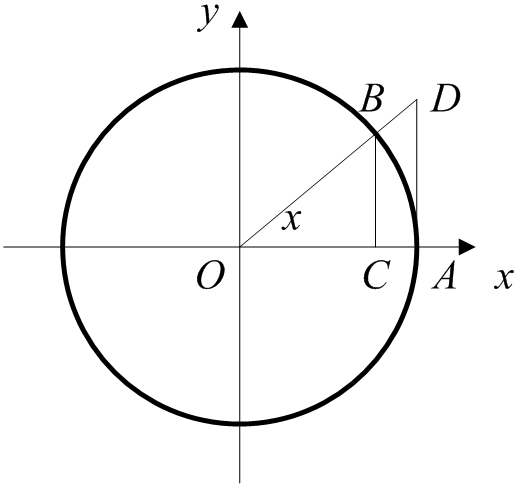
\includegraphics[height=3.5cm]{1.1.png}
\end{figure}

考虑单位圆,{\it OD}和{\it x}轴夹角 。
考察三角形{\it OBC}、扇形{\it OAB}、三角形{\it OAD},三者面积有关系:
\begin{align*}
&\because S_{OBC}<S_{OAB}<S_{OAD} \\
&\therefore \frac{1}{2}\sin x\cos x<\pi \cdot \frac{x}{2\pi}<\frac{1}{2}\tan x \\
&\therefore \cos x<\frac{\sin x}{x}<\frac{1}{\cos x}
\end{align*}
对于余弦函数有$\underset{x\rightarrow 0}{\lim}\cos x=1$,由夹逼定理得:
\[
\underset{x\rightarrow 0}{\lim}\frac{\sin x}{x}=1
\]

注意,这里不能用线段{\it BC}长度、弧{\it AB}长度、线段{\it AD}长度的关系$BC<\overset\frown{AB}<AD$。
因为$\overset\frown{AB}<AD$不是那么显而易见,需要证明。

\begin{tcolorbox}
该极限将三角函数和多项式函数联系起来。
其值是一个计算得到的数值。
\end{tcolorbox}

{\bf 计算$\underset{x\rightarrow \infty}{\lim}\left( 1+\frac{1}{x} \right) ^x$}

还是用夹逼定理。
构造一个数列$x_n=\left( 1+\frac{1}{n} \right) ^n$。
用有界定理推导极限$\underset{n\rightarrow \infty}{\lim}\left\{ x_n \right\} $存在,证明略,并记为$e$。
\begin{align*}
&\because x>0\Rightarrow n\leqslant x\leqslant n+1 \\
&\therefore \left( 1+\frac{1}{1+n} \right) ^n<\left( 1+\frac{1}{x} \right) ^n\leqslant \left( 1+\frac{1}{x} \right) ^x\leqslant \left( 1+\frac{1}{n} \right) ^x<\left( 1+\frac{1}{n} \right) ^{n+1} \\
&\because \begin{cases}
	\underset{n\rightarrow \infty}{\lim}\left( 1+\frac{1}{1+n} \right) ^n=\underset{n\rightarrow \infty}{\lim}\frac{\left( 1+\frac{1}{1+n} \right) ^{n+1}}{1+\frac{1}{1+n}}=e\\
	\underset{n\rightarrow \infty}{\lim}\left( 1+\frac{1}{n} \right) ^{1+n}=\underset{n\rightarrow \infty}{\lim}\left[ \left( 1+\frac{1}{1+n} \right) ^n\left( 1+\frac{1}{1+n} \right) \right] =e\\
\end{cases} \\
&\therefore \underset{x\rightarrow +\infty}{\lim}\left( 1+\frac{1}{x} \right) ^x=e
\end{align*}
同理可证明$\underset{x\rightarrow -\infty}{\lim}\left( 1+\frac{1}{x} \right) ^x=e$。
由左右极限存在且相等得该极限存在且:
\[
\underset{x\rightarrow \infty}{\lim}\left( 1+\frac{1}{x} \right) ^x
\]

\begin{tcolorbox}
注意,该极限的值$e$是一个定义值。
该极限把指数函数和幂函数联系起来。
对于幂指函数的极限,基本都会有$e$的影子。
\end{tcolorbox}






\newpage
\section{无穷小量和无穷大量}

本节给出无穷小量的概念,是微分的基础概念。

本节要点:
\begin{itemize}
    \item 理解无穷小量和无穷大量的概念;
    \item 理解本节最后一条定理。
\end{itemize}

%============================================================
\subsection{无穷量的概念}

\begin{definition}[无穷小量]
若$\forall \varepsilon >0$时存在$\delta >0$,当$x\in N\left( \hat{x}_0,\delta \right) $时有$\left| f\left( x \right) -0 \right|<\varepsilon $,则称$f\left( x \right) $为{\bf 当$x\rightarrow x_0$时的无穷小量},记作
\[
\underset{x\rightarrow x_0}{\lim}f\left( x \right) =0
\]
\end{definition}

注意:0是一个特殊的无穷小量,也是唯一可以作为无穷小量的常数。

\begin{definition}[无穷大量]
若$\forall M>0$时存在$\delta >0$,当$x\in N\left( \hat{x}_0,\delta \right) $时有$\left| f\left( x \right) -0 \right|>M$,则称$f\left( x \right) $为{\bf 当$x\rightarrow x_0$时的无穷大量},记作
\[
\underset{x\rightarrow x_0}{\lim}f\left( x \right) =\infty
\]
\end{definition}

本质上,无穷小量和无穷大量都是极限,是函数的趋势。

%============================================================
\subsection{无穷量的定理}

\begin{theorem}[互倒定理]
在自变量趋向一致下,无穷小量和无穷大量互为倒数。
\end{theorem}

\begin{theorem}[有限和定理]
有限个无穷小量之和(差)仍为无穷小量。
\end{theorem}

\begin{theorem}[有限积定理]
有限个无穷小量之积仍为无穷小量。
\end{theorem}

\begin{theorem}[有界积定理]
若$\underset{x\rightarrow x_0}{\lim}f\left( x \right) =0$,$g\left( x \right) $在$x_0$的某去心邻域内有界,则$\underset{x\rightarrow x_0}{\lim}\left[ f\left( x \right) \cdot g\left( x \right) \right] =0$。
\end{theorem}

\begin{theorem}
$\underset{x\rightarrow x_0}{\lim}f\left( x \right) =A\Leftrightarrow f\left( x \right) =A+o\left( x \right) $,其中$A$为常数,$o\left( x \right) $为无穷小量,即$\underset{x\rightarrow x_0}{\lim}o\left( x \right) =0$。
\end{theorem}

最后一条定理反映的是极限运算,也是后续微分和近似分析的基础。

%============================================================
\subsection{无穷小的比较}

\begin{definition}
设$\underset{x\rightarrow x_0}{\lim}\alpha \left( x \right) =0,\underset{x\rightarrow x_0}{\lim}\beta \left( x \right) =0,\beta \left( x \right) \ne 0$ ,则可有如下定义:
\begin{itemize}
    \item 若有$\underset{x\rightarrow x_0}{\lim}\frac{\alpha \left( x \right)}{\beta \left( x \right)}=0$,则称当$x\rightarrow x_0$时,{\bf $\alpha \left( x \right) $是$\beta \left( x \right) $的高阶无穷小量},或{\bf $\beta \left( x \right) $是$\alpha \left( x \right) $的低阶无穷小量},记作$\alpha \left( x \right) =o\left( \beta \left( x \right) \right) $,
    \item 若有$\underset{x\rightarrow x_0}{\lim}\frac{\alpha \left( x \right)}{\beta \left( x \right)}=C\ne 0$,则称当$x\rightarrow x_0$时,{\bf $\alpha \left( x \right) $和$\beta \left( x \right) $是同阶无穷小量},特别地,如$C=1$,则称{\bf $\alpha \left( x \right) $和$\beta \left( x \right) $是等价无穷小},记作$\alpha \left( x \right) \sim \beta \left( x \right) $,
    \item 若$\underset{x\rightarrow x_0}{\lim}\frac{\alpha \left( x \right)}{\left[ \beta \left( x \right) \right] ^k}=C\ne 0,k>0$则称当$x\rightarrow x_0$时,{\bf $\alpha \left( x \right) $是$\beta \left( x \right) $的$k$阶无穷小量}。
\end{itemize}
\end{definition}

无穷小量的比较的数学意义是描述谁的趋近速度快。






\newpage
\section{光滑曲线的第一个要求}

对于好函数的要求——光滑,我们第一个直觉是“不能断”。

\begin{figure}[h]
\centering
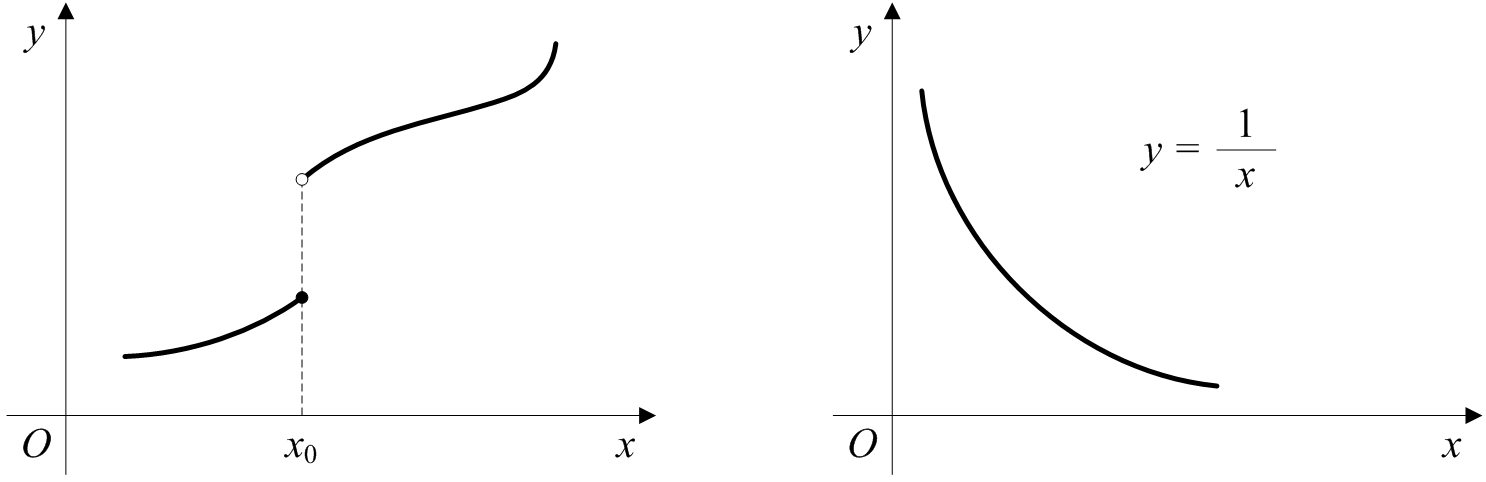
\includegraphics[height=3cm]{1.2.png}
\end{figure}

左上图的曲线不光滑,它“断了”。
右上图的曲线咋看没问题,但是在$x=0$处断了,不是人为地断,而是这个函数根本到不了断点。

那么什么是断,什么又不是断,我们需要给出一个数学上的“不断”的定义——连续。






\newpage
\section{连续}

本节给出的函数连续的定义,并给出连续的运算和定理。
最重要的是根据定理推导的一个重要的极限。

本节要点:
\begin{itemize}
    \item 理解连续的概念;
    \item 推导一个重要的极限:$\underset{x\rightarrow 0}{\lim}\frac{a^x-1}{x}=\ln a$。
\end{itemize}

%============================================================
\subsection{连续的概念}

\begin{definition}[连续]
设$f\left( x \right) $在某邻域$N\left( x_0 \right) $内有定义,若
\[
\underset{x\rightarrow x_0}{\lim}f\left( x \right) =f\left( x_0 \right)
\]
则称{\bf $f\left( x \right) $在点$x_0$处连续(continuity)}。
\end{definition}

连续在数学上规范了什么是“不断”。

\begin{definition}[区间连续]
若$f\left( x \right) $在开区间$\left( a,b \right) $内每一点连续,则称{\bf $f\left( x \right) $在开区间$\left( a,b \right) $连续},$\left( a,b \right) $称为$f\left( x \right) $的{\bf 连续区间},我们将$C\left( a,b \right) $表示$\left( a,b \right) $上所有连续函数构成的集合,则$f\left( x \right) \in C\left( a,b \right) $;若$f\left( x \right) $在开区间$\left( a,b \right) $连续,在点$a$右连续,在点$b$左连续,则称{\bf $f\left( x \right) $在闭区间$\left[ a,b \right] $连续}。
\end{definition}

\begin{definition}[一致连续性]
上面区间连续的定义中,当考察$\left| x-x_0 \right|<\delta $时,显然$\delta $可以和$x_0$有关。
当我们更严格地规定$\delta $仅和$\varepsilon $有关,与$x_0$具体在哪里无关时,称为$f\left( x \right) $在区间$\left( a,b \right) $(或$\left[ a,b \right] $){\bf 一致连续},或称{\bf 均匀连续}。
\end{definition}

\begin{definition}[间断点]
若$f\left( x \right) $在点$x_0$处不连续,则称$x_0$为$f\left( x \right) $的{\bf 间断点}。
\begin{itemize}
    \item 若$f\left( x \right) $在间断点$x_0$处左右极限均存在,称$x_0$为$f\left( x \right) $的{\bf 第一类间断点},
    \begin{itemize}
        \item 当左右极限不相等时,称为{\bf 跳跃型间断点},
        \item 当左右极限相等,但$x_0$未定义或$\underset{x\rightarrow x_0}{\lim}f\left( x \right) \ne f\left( x_0 \right) $时,称为{\bf 可去型间断点};
    \end{itemize}
    \item 反之,若$f\left( x \right) $在间断点$x_0$处左右极限均不存在,或有一个不存在,称$x_0$为$f\left( x \right) $的{\bf 第二类间断点},
    \begin{itemize}
        \item 当有某侧极限为无穷大时,称为{\bf 无穷型间断点},
        \item 当某一侧极限呈振荡,不收敛于一个值时,称为{\bf 振荡型间断点}。
    \end{itemize}
\end{itemize}
\end{definition}

间断点表示函数不连续,第一类间断点表示函数还是往那个值收敛的,第二类间断点则表示函数在那个点是发散的。
第一类间断点对积分没有影响,第二类间断点就可能无法积分了。

%============================================================
\subsection{连续的几何意义}

几何上,连续表示从一点画到另一点,笔不能离开纸面。
也就是说,变量从一个量到另一个量,必然通过中间的某个量。
再看下面两个断的曲线。
左图在$x=x_0$时是有值的,但是笔在该点腾空了,反映在连续上,左右连续不是相等的。
右图在$x=0$时函数根本没有极限,或者说极限为$\infty $。

\begin{figure}[h]
\centering
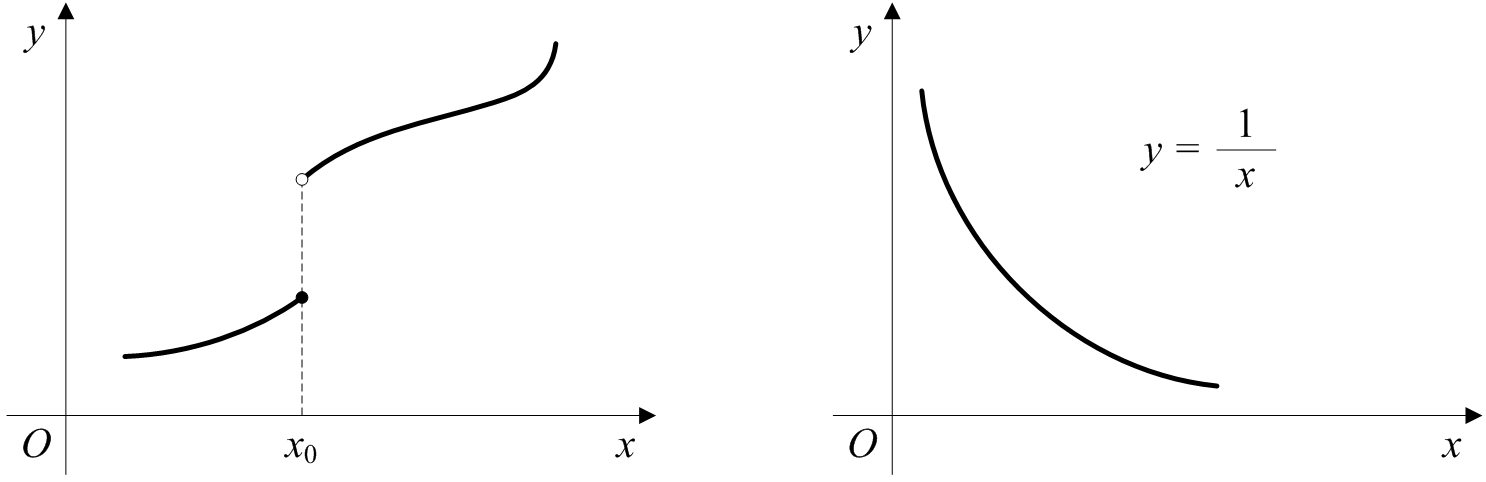
\includegraphics[height=3cm]{1.2.png}
\end{figure}

基于这个几何意义,连续的运算法则和几个定理也是非常容易理解,且不证自明。

%============================================================
\subsection{连续的运算法则}

若$f\left( x \right) ,g\left( x \right) $在点$x_0$处连续,则有
\begin{align*}
&C\cdot f\left( x \right) \\
&f\left( x \right) \pm g\left( x \right) \\
&f\left( x \right) \cdot g\left( x \right) \\
&\frac{f\left( x \right)}{g\left( x \right)}
\end{align*}
且在点$x_0$处连续。
特别注意1、2两式表明连续也是线性的。

%============================================================
\subsection{连续的定理}

\begin{theorem}[初等函数连续定理]
基本初等函数和初等函数在其定义域的区间上是连续的。
\end{theorem}

\begin{theorem}[反函数的连续性]
若函数$f\left( x \right) $在某区间内连续且单调,则其反函数$f^{-1}\left( x \right) $在原函数对应的值域内连续且单调,且具有相同的单调性。
\end{theorem}

\begin{theorem}[复合函数的连续性]
若$\underset{x\rightarrow x_0}{\lim}\varphi \left( x \right) =\varphi \left( x_0 \right) =u_0$,$\underset{u\rightarrow u_0}{\lim}f\left( u \right) =f\left( u_0 \right) $,则
\[
\underset{x\rightarrow x_0}{\lim}f\left( \varphi \left( x \right) \right) =f\left( \underset{x\rightarrow x_0}{\lim}\varphi \left( x \right) \right) =f\left( \varphi \left( x_0 \right) \right)
\]
\end{theorem}

该定理表示极限符号和函数符号可以交换顺序。
初等函数连续定理和该定理常用于计算极限。

\begin{theorem}[最值定理]
若$f\left( x \right) $在闭区间$\left[ a,b \right] $连续,则必在$\left[ a,b \right] $上有最大值和最小值。
\end{theorem}

\begin{theorem}[有界定理]
若$f\left( x \right) $在闭区间$\left[ a,b \right] $连续,则必在$\left[ a,b \right] $上有界。
\end{theorem}

\begin{theorem}[介值定理]
若$f\left( x \right) $在闭区间$\left[ a,b \right] $连续,且$f\left( a \right) \ne f\left( b \right) $,则对于任何$\forall \mu \in \left[ f\left( a \right) ,f\left( b \right) \right] $或$\forall \mu \in \left[ f\left( b \right) ,f\left( a \right) \right] $,必存在$\xi \in \left[ a,b \right] $,使得$f\left( \xi \right) =\mu $。几何上表示曲线$y=f\left( x \right) $和直线$y=\mu $至少有一个交点。
\end{theorem}

\begin{corollary}
若$f\left( x \right) $在闭区间$\left[ a,b \right] $连续,且有最大值和最小值$m,M$,则对于任何$\forall \mu \in \left[ m,M \right] $,必存在$\xi \in \left[ a,b \right] $,使得$f\left( \xi \right) =\mu $。
\end{corollary}

\begin{corollary}[根存在定理]
若$f\left( x \right) $在闭区间$\left[ a,b \right] $连续,且$f\left( a \right) \cdot f\left( b \right) <0$,则必存在$\xi \in \left[ a,b \right] $,使得$f\left( \xi \right) =0$。
\end{corollary}

\begin{corollary}[唯一根存在定理]
若$f\left( x \right) $在闭区间$\left[ a,b \right] $连续且严格单调,且$f\left( a \right) \cdot f\left( b \right) <0$,则有唯一$\xi \in \left[ a,b \right] $,使得$f\left( \xi \right) =0$。
\end{corollary}

最值定理和有界定理是等价的。

%============================================================
\subsection{两个重要的极限}

{\bf 计算$\underset{x\rightarrow 0}{\lim}\frac{\log _a\left( 1+x \right)}{x}$}

首先有
\[
\frac{\log _a\left( 1+x \right)}{x}=\log _a\left( 1+x \right) ^{\frac{1}{x}}
\]
然后运用复合函数的连续性定理:
\[
\underset{x\rightarrow 0}{\lim}\log _a\left( 1+x \right) ^{\frac{1}{x}}=\log _a\underset{x\rightarrow 0}{\lim}\left( 1+x \right) ^{\frac{1}{x}}=\log _ae=\frac{\ln e}{\ln a}=\frac{1}{\ln a}
\]
特别的,当$a=e$时:
\[
\underset{x\rightarrow 0}{\lim}\frac{\ln \left( 1+x \right)}{x}=1
\]

{\bf 计算$\underset{x\rightarrow 0}{\lim}\frac{a^x-1}{x}$}

令$a^x-1=t$,得$x=\log _a\left( t+1 \right) $,且$x\rightarrow 0$时有$t\rightarrow 0$,所以:
\[
\underset{x\rightarrow 0}{\lim}\frac{a^x-1}{x}=\underset{x\rightarrow 0}{\lim}\frac{t}{\log _a\left( t+1 \right)}=\underset{x\rightarrow 0}{\lim}\frac{1}{\log _a\left( t+1 \right) ^{1/t}}=\ln a
\]
特别的,当$a=e$时:
\[
\underset{x\rightarrow 0}{\lim}\frac{e^x-1}{x}=1
\]

\begin{tcolorbox}
该极限在求解指数函数$a^x$的导数时用到,是三大基本导数之一。
\end{tcolorbox}

%============================================================
\subsection{再论四个重要极限}

以下四个重要极限揭示了基本初等函数之间的关系:

\begin{table}[h]
\centering
\begin{tabular}{lc}
    \toprule
    极限 & 函数间的联系\\
    \midrule
    $\underset{x\rightarrow 0}{\lim}\frac{\sin x}{x}=1$ & 联系了幂函数和三角函数。\\
    $\underset{x\rightarrow \infty}{\lim}\left( 1+\frac{1}{x} \right) ^x=e$ & 联系了幂函数和指数函数。\\
    $\underset{x\rightarrow 0}{\lim}\frac{\log _a\left( 1+x \right)}{x}=\frac{1}{\ln a}$ & 联系了幂函数和对数函数。\\
    $\underset{x\rightarrow 0}{\lim}\frac{a^x-1}{x}=\ln a$ & 联系了幂函数和指数函数。\\
    \bottomrule
\end{tabular}
\end{table}






\newpage
\section{本章小结}

形而下来讲,本章最重要的概念是“极限”及其运算,是后续章节的基础。
形而上来讲,本章最重要的是“连续”。
因为我们的目标是理解“光滑”的好函数。
什么是光滑,通过连续这个数学概念,严格地、量化地规定了光滑的第一个要求——不断。






\newpage
\section{习题}

\begin{exercise}
求下列极限:
\begin{enumerate}
    \item $\underset{x\rightarrow -2}{\lim}\frac{x^2-x+2}{x^2+4}$
    \item $\underset{x\rightarrow 1}{\lim}\left( \frac{1}{1-x}-\frac{3}{1-x^2} \right) $
    \item $\underset{x\rightarrow 0}{\lim}\frac{\left| 2x-1 \right|-\left| 2x+1 \right|}{x}$
    \item $\underset{x\rightarrow 0}{\lim}\frac{x-\sin 2x}{x+\sin 5x}$
    \item $\underset{x\rightarrow \infty}{\lim}\left( \frac{x-4}{x+1} \right) ^{2x-1}$
    \item $\underset{x\rightarrow \infty}{\lim}\sin \left( 1+\frac{1}{x} \right) ^{2x+1}$
    \item $\underset{x\rightarrow \infty}{\lim}\lg \frac{100+x^2}{1+100x^2}$
\end{enumerate}
\end{exercise}

解:

1.
\[
\underset{x\rightarrow -2}{\lim}\frac{x^2-x+2}{x^2+4}=\left. \frac{x^2-x+2}{x^2+4} \right|_{x=-2}=1
\]

2.
\[
\underset{x\rightarrow 1}{\lim}\left( \frac{1}{1-x}-\frac{3}{1-x^2} \right) =\underset{x\rightarrow 1}{\lim}\frac{\left( x+2 \right) \left( x-1 \right)}{1-x^3}=-\underset{x\rightarrow 1}{\lim}\frac{x+2}{x^2+x+1}=-1
\]

3.
\[
\underset{x\rightarrow 0}{\lim}\frac{\left| 2x-1 \right|-\left| 2x+1 \right|}{x}=\underset{x\rightarrow 0}{\lim}\frac{\left( 1-2x \right) -\left( 2x+1 \right)}{x}=\underset{x\rightarrow 0}{\lim}\frac{-4x}{x}=-4
\]

4.
\[
\underset{x\rightarrow 0}{\lim}\frac{x-\sin 2x}{x+\sin 5x}=\underset{x\rightarrow 0}{\lim}\frac{1-2\frac{\sin 2x}{2x}}{1+5\frac{\sin 5x}{5x}}=-\frac{1}{6}
\]

5.
\begin{align*}
&\underset{x\rightarrow \infty}{\lim}\left( \frac{x-4}{x+1} \right) ^{2x-1}=\underset{x\rightarrow \infty}{\lim}\left( 1+\frac{-5}{x+1} \right) ^{2\left( x+1 \right) -3} \\
&=\underset{x\rightarrow \infty}{\lim}\left( 1+\frac{-10}{2\left( x+1 \right)} \right) ^{2\left( x+1 \right)}\cdot \underset{x\rightarrow \infty}{\lim}\left( 1-10\frac{1}{2\left( x+1 \right)} \right) ^{-3} \\
&=\underset{t\rightarrow \infty}{\lim}\left( 1+\frac{-10}{t} \right) ^t\cdot 1^{-3}=e^{-10}
\end{align*}

6.
\begin{align*}
&\underset{x\rightarrow \infty}{\lim}\sin \left[ \left( 1+\frac{1}{x} \right) ^{2x+1} \right] =\sin \underset{x\rightarrow \infty}{\lim}\left( 1+\frac{2}{2x} \right) ^{2x+1} \\
&=\sin \left[ \underset{x\rightarrow \infty}{\lim}\left( 1+\frac{2}{2x} \right) ^{2x}\cdot \underset{x\rightarrow \infty}{\lim}\left( 1+\frac{2}{2x} \right) ^1 \right] =\sin \left( e^2\cdot 1 \right)
\end{align*}

7.
\[
\underset{x\rightarrow \infty}{\lim}\lg \frac{100+x^2}{1+100x^2}=\lg \underset{x\rightarrow \infty}{\lim}\frac{100+x^2}{1+100x^2}=\lg \frac{1}{100}=-2
\]

\begin{tcolorbox}
本题还是以直接带入为主,有些小题需要化简一下式子而已。
\end{tcolorbox}

~

\begin{exercise}
求$\underset{x\rightarrow +\infty}{\lim}\left( \sin \sqrt{x+1}-\sin \sqrt{x} \right) $。
\end{exercise}

解:

总体思路是将两个三角函数合并到一个,然后考察三角函数内多项式的极限。

首先化简三角函数:
\[
\underset{x\rightarrow +\infty}{\lim}\left( \sin \sqrt{x+1}-\sin \sqrt{x} \right) =\underset{x\rightarrow +\infty}{\lim}2\cos \frac{\sqrt{x+1}+\sqrt{x}}{2}\sin \frac{\sqrt{x+1}-\sqrt{x}}{2}
\]
然后考察$\cos \frac{\sqrt{x+1}+\sqrt{x}}{2}$,是有界函数,再考察$\sin \frac{\sqrt{x+1}-\sqrt{x}}{2}$,当$x\rightarrow \infty $时似乎$\sqrt{x+1}-\sqrt{x}\rightarrow 0$:
\begin{align*}
&\because \frac{\sqrt{x+1}-\sqrt{x}}{2}=\frac{1}{2\left( \sqrt{x+1}+\sqrt{x} \right)} \\
&\therefore \underset{x\rightarrow +\infty}{\lim}\sin \frac{\sqrt{x+1}-\sqrt{x}}{2}=\sin \underset{x\rightarrow +\infty}{\lim}\frac{1}{2\left( \sqrt{x+1}+\sqrt{x} \right)}=\sin 0=0
\end{align*}
所以:
\[
\underset{x\rightarrow +\infty}{\lim}\left( \sin \sqrt{x+1}-\sin \sqrt{x} \right) =\underset{x\rightarrow +\infty}{\lim}\left( 2\cos \frac{\sqrt{x+1}+\sqrt{x}}{2}\cdot 0 \right) =0
\]

~

\begin{exercise}
若
\[
\begin{cases}
	\underset{x\rightarrow a}{\lim}\left[ f\left( x \right) +g\left( x \right) \right] =2\\
	\underset{x\rightarrow a}{\lim}\left[ f\left( x \right) -g\left( x \right) \right] =1\\
\end{cases}
\]
求$\underset{x\rightarrow a}{\lim}\left[ f\left( x \right) \cdot g\left( x \right) \right] $。
\end{exercise}

解:

总体思路是采用极限的线性组合。
\begin{align*}
&\because \begin{cases}
	\underset{x\rightarrow a}{\lim}\left[ f+g \right] ^2=\underset{x\rightarrow a}{\lim}\left[ f^2+g^2+2fg \right] =4\\
	\underset{x\rightarrow a}{\lim}\left[ f-g \right] ^2=\underset{x\rightarrow a}{\lim}\left[ f^2+g^2-2fg \right] =1\\
\end{cases} \\
&\therefore \underset{x\rightarrow a}{\lim}fg=\frac{1}{4}\left( 4-1 \right) =\frac{3}{4}
\end{align*}

~

\begin{exercise}
若有方程$x^3-3x=1$,讨论其在$\left[ 1,2 \right] $上有无根。
\end{exercise}

解:

总体思路是考察连续函数的根存在定理。

令$y=x^3-3x-1$,则$y$在$\left[ 1,2 \right] $上连续,且:
\[
y\left( 1 \right) \cdot y\left( 2 \right) =-3<0
\]
根据根存在定理,必有根。

~

\begin{exercise}
如下图,等边三角形内放置直径相同的若干个圆,图示为10个,三角形外切圆。当增大圆的个数时,能否覆盖三角形,如能则最终需要多少个,如不能,则最终能覆盖多少三角形面积。
\begin{figure}[h]
\centering
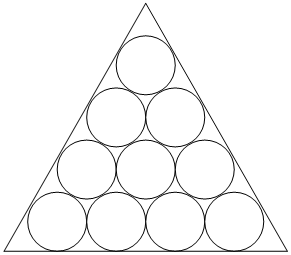
\includegraphics[height=2.5cm]{1.3.png}
\end{figure}
\end{exercise}

解:

总体思路是考察圆的总面积和三角形面积的比例的极限。

假设三角形面积$A$,所有圆面积之和$A_n$,圆半径$r$,一边放$n$个,一共$\frac{1}{2}n\left( n-1 \right) $个圆。于是所有圆面积之和$A_n$为:
\[
A_n=\pi r^2\cdot \frac{1}{2}n\left( n+1 \right)
\]
易得三角形边长$L=2\left( n-1 \right) r+2\sqrt{3}\cdot r$,于是三角形面积$A$为:
\[
A=\frac{1}{2}\cdot L\cdot \frac{\sqrt{3}}{2}L=\frac{\sqrt{3}}{4}\left[ 2\left( n-1 \right) r+2\sqrt{3}r \right] ^2
\]
于是:
\[
\underset{n\rightarrow \infty}{\lim}\frac{A_n}{A}=\underset{n\rightarrow \infty}{\lim}\frac{\pi r^2\cdot \frac{1}{2}n\left( n+1 \right)}{\frac{\sqrt{3}}{4}\left[ 2\left( n-1 \right) r+2\sqrt{3}r \right] ^2}=\frac{\pi r^2\cdot \frac{1}{2}}{\frac{\sqrt{3}}{4}\cdot 4r^2}=\frac{\pi}{2\sqrt{3}}=0.9069
\]
最多只能覆盖三角形的90\%多一点的面积。









